\documentclass{report}

\usepackage{float}
\usepackage{url}
\usepackage{graphicx}
\usepackage{listings}
\usepackage{color}
\usepackage{verbatim}
\usepackage[lined,linesnumbered,algochapter]{algorithm2e}
\usepackage{tikz}
\usetikzlibrary{arrows,automata}
\usepackage{xspace}
\usepackage{caption}
%\usepackage[colorlinks = true, urlcolor  = blue]{hyperref}
\usepackage{ucs}
\usepackage[utf8]{inputenc}

%\hypersetup{colorlinks=false, linkcolor=red}

\usepackage{ngerman}
\usepackage[ngerman, english]{babel}
\usepackage{bibgerm,cite}       % Deutsche Bezeichnungen, Automatisches Zusammenfassen von Literaturstellen
\usepackage[ngerman]{varioref}  % Querverweise

\DeclareCaptionFont{white}{\color{white}}
\DeclareCaptionFormat{listing}{\colorbox{gray}{\parbox{\textwidth}{#1#2#3}}}
\captionsetup[lstlisting]{format=listing,labelfont=white,textfont=white}

\lstset{language=Java,captionpos=b,tabsize=3,frame=lines,keywordstyle=\color{blue},commentstyle=\color{darkgreen},stringstyle=\color{red},numbers=left,numberstyle=\tiny,numbersep=5pt,breaklines=true,showstringspaces=false,basicstyle=\footnotesize,emph={label}}

\setcounter{secnumdepth}{2}
\setcounter{tocdepth}{3}

% another code presentation stlye
%\definecolor{dkgreen}{rgb}{0,0.6,0}
%\definecolor{gray}{rgb}{0.5,0.5,0.5}
%\definecolor{mauve}{rgb}{0.58,0,0.82}
%
%\lstset{frame=tb,
%  language=Java,
%  aboveskip=3mm,
%  belowskip=3mm,
%  showstringspaces=false,
%  columns=flexible,
%  basicstyle={\small\ttfamily},
%  numbers=none,
%  numberstyle=\tiny\color{gray},
%  keywordstyle=\color{blue},
%  commentstyle=\color{dkgreen},
%  stringstyle=\color{mauve},
%  breaklines=true,
%  breakatwhitespace=true
%  tabsize=3
%}

% define custom macros for specific formats or names
\newcommand{\uml}[1]{\texttt{#1}}
\newcommand{\cd}{\textsf{Class Diagram}}

\begin{document}
\pagestyle{plain}
\pagenumbering{roman}

\title{Risikomanagement}


\maketitle

\tableofcontents
\newpage

\pagenumbering{arabic}

% Kapitel
% --------------------------------------------------------------
\chapter{Definition und Grundlagen Risikomanagement}
\label{sect:grundlagen}


% --------------------------------------------------------------
\chapter{Software, Plattformen und Apps im Risikomanagement}

\section{Einleitung}

In den letzten Jahren wurde viel in die Entwicklung von Systemen die Risiko messbar machen investiert. Risikomessung ist stets eine passive Aktivität. Risikomanagement ist ein dynamisches bestreben und benötigt Tools und Anwendungen die beim identifizieren und verringern der Risikoquellen helfen. \cite{Mausser1997} 
NASA ist wegweisend in diesem Bereich. Die Steuerung von Risiko wird als Resource angesehen die gehandelt werden kann gegen andere Resourcen wie Zeit, Kosten oder Leistung. Ein erfolgreiches Risikomanagement beinhaltet also das Identifizieren des Risikos, das Abschätzen der Auswirkungen und der Eintrittswahrscheinlichkeit, das Entscheiden welche Risiko-level akzeptabel sind und die Risikominimierung.\cite{Feather2000}

In den Anfangsphasen eines Projektes ist Risikomanagement hauptsächlich qualitativ. Basierend auf den vorhandenen Informationen sind die Risiken kategorisiert und normalerweise high-level. In späteren Phasen geht es mehr um Teilsysteme, Detailanforderungen und Herstellungs / Softwaremodelle. Risikomanagement ist jetzt primär quantitativ und nicht qualitativ. Die identifizierten Risiken sind sehr detailliert und fokussiert auf spezifische Probleme.\cite{Feather2000}


\section{Kategorien}

Um eine ordentliche Analyse durchzuführen ist es wichtig die Vorteile und Nachteile von Quantitativen und Qualitativen Risiken zu beachten.\cite{Stoneburner2002}

\subsection{Qualitativ}
Der groeste Vorteil von qualitativer Risikoanalyse ist das die Risiken priorisiert werden und bereits mögliche Verbesserungen in Betracht gezogen werden.
Mit der qualitativen Analyse ist is dafür schwierig abzuschätzen welche Kostenvorteile gewisse Gegenmaßnahmen haben, da keine messbaren Werte fuer das Ausmass der Risiken vorhanden sind.\cite{Stoneburner2002}
\subsection{Quantitativ}
Der Vorteil von quantitativer Risikoanalyse ist das es die Messbarkeit fuer das Ausmass von Risiken verbessert. Dadurch können die Kostenvorteile von Gegenmaßnahmen besser analysiert werden.
Im Gegensatz zur qualitativen Analyse ist das interpretieren der quantitativen Analyse schwieriger. Abhängig von den gemessenen Werten kann es sein das weitere Faktoren in Betracht gezogen werden muessen um die Ergebnisse zu verstehen.\cite{Stoneburner2002}

\subsection{Kombiniere Qualitativ und Quantitativ}
Sowohl die Qualitative als auch Quantitative Methode haben ihr Vorteile und Nachteile. Um auf ein gutes Ergebnis der Risikoanalyse zu kommen können beide kombiniert werden. Dadurch werden die Informationen im Gesamtbild betrachtet und eine Interpretation der Daten wird vereinfacht. Als Beispiel gilt hier das von der NASA verwendete Risk Balancing Profile fuer qualitative Daten und Defect Detection and Prevention fuer quantitative Daten. In \cite{Feather2000} werden diese beiden Tools vorgestellt und dargelegt wie eine Kombination daraus aussieht.

\section{Tools}
\subsection{Appthority}

\subsubsection{Beschreibung}
Appthority wurde 2011 gegründet mit einem einzigen Ziel, Firmen vor Sicherheits-, Datenverlust- und Privatsphäre Risiken zu schützen die durch schnell wachsende Mitarbeiterzahlen und die daraus resultierende Verwendung von mobilen Anwendungen entsteht. Es bietet eine einfache und skalierbare Möglichkeit diese Risiken zu beherrschen.\cite{AppthorityBlog}\cite{Appthority}

\begin{enumerate}
\item Die Appthority Datenbank beinhaltet mehr als 3 Millionen Anwendungen.
\item Vorerst nur iOS und Android unterstützt.
\item Blackberry 10 und Windows Phone apps sollen folgen.
\item Über 1 Millionen API Anfragen pro Tag
\end{enumerate}

\subsubsection{Anwendung}
Bis 2013 gab es bei Appthority nur die Möglichkeit über eine API die analysierten Daten zu erhalten. Seit 2 Jahren gibt es nun ein Webportal das ebenfalls dafür genutzt werden kann. An dieser zentralen Stelle kann fuer alle mobilen Geräte die von den Mitarbeitern einer Firma im Umlauf sind eine Riskoanalyse durchgeführt werden. Dabei werden sämtliche sich auf den Geräten befindenden Anwendungen mit der jeweiligen Versionsnummer von Appthority kontrolliert. Befinden sich potentiell gefährliche Anwendungen auf einem Gerät, werden die zuständigen IT Fachkräfte darüber informiert. \ref{fig:appthority} \cite{AppthorityBlog}\cite{Appthority}

\subsubsection{Appthorities Analyse}
\begin{enumerate}
\item Statische und dynamische Analyse des Binaerfiles 
\item Über 3000 Regeln die kontrolliert werden
\item Wie verhält sich die Anwendung?
\item Aus welchem Land kommt die Anwendung?
\item Von welchen Entwicklern wurde die Anwendung entwickelt?
\item Welchen anderen Referenzen haben diese Entwickler?
\end{enumerate}

\begin{figure}[h!]
  \centering
  \fbox{
    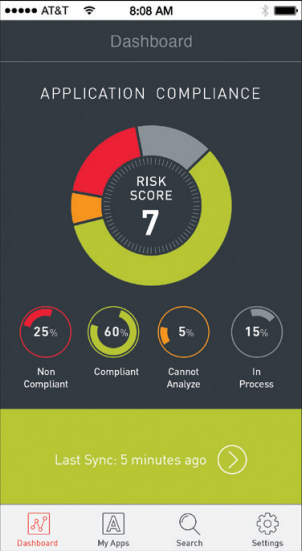
\includegraphics[width=0.4 \textwidth]{./Images/appthority.png}
  }
  \caption{Appthority}
  \label{fig:appthority}
\end{figure}

\subsection{IntelliRisk}
\subsubsection{Beschreibung}

IntelliRisk ist ein Produkt der American International Group, einer der international führenden Versicherungsorganisation tätig in über 130 Ländern. Es bietet schnellen und einfachen Zugang zu Informationen und die Möglichkeit Reports zu erstellen. AIG bietet auch eine erweiterte Variante mit dem Namen IntelliRisk Advanced an. Diese verfügt über komplexere Risiko und Forderungsfeatures.\cite{AIG}
\begin{enumerate}
\item interaktives Dashboard
\item real-time Zugriff auf Aktivitätsnotizen
\item Alarmsystem bei signifikanten Veraenderungen
\item konfigurierbare Reports
\item Identifikation von hohen Kosten
\item mobile Version
\end{enumerate}


\subsection{SaS for Enterprise Risk Management}
\subsubsection{Beschreibung}
SAS bietet durchgängige Softwarelösungen für den gesamten Prozess des Risikomanagements. Angefangen von der Datenaufbereitung bis über Risikokalkulation, Aggregation und Reporting. Egal ob Finanzkennzahlen, Produkt- und Kundendaten, Marktinformationen oder operative Messgrößen, mit SAS werden die enormen Datenmengen aus allen operativen Systemen integriert und für die Risikosteuerung nutzbar. Korrelationen zwischen Risikoarten werden sichtbar und verbessern den Umgang damit.

\begin{enumerate}
\item Nachweis der ordnungsgemäßen Umsetzung der GRC-Regularien.
\item Echtzeit Dashboard
\item Alarmsystem
\end{enumerate}

\subsection{IntelligenceBank GRC}

\subsubsection{Beschreibung}
IntelligenceBank GRC ist eine Platform as a Service Lösung aus Australien. Risikomanager können innerhalb dieser Platform Risiken, Vorfälle und andere firmen interne Daten eintragen. Diese analysierten und aufgeschlüsselten Daten können dem Firmenmanagement und Stakeholdern präsentiert werden, die somit jederzeit einen klaren Überblick über aktuelle Risiken und deren Status haben.
\subsubsection{Anwendung}
In der Webanwendung ist die Register-Ansicht eine der wichtigsten. Die bereits vorhandenen wie Risiko, Gesundheit, Vertrag, Unfälle oder Kunden können nach belieben erweitert werden um den jeweiligen Anforderungen zu entsprechen. Zu jedem dieser Register gehört ein bestimmter Eingabeprozess der angepasst werden kann.\cite{intelligencebank}

\subsection{Citicus MOCA}
\subsubsection{Beschreibung}
Im Unterschied zu den bis jetzt angeführten Lösungen ist Citicus MOCA eine reine iPhone Anwendung. Die App laesst den Benutzer alle möglichen beeinflussenden Faktoren eintragen und diese bewerten, um anschliessend ein Ergebnis daraus zu ziehen.\cite{Citicus}

\begin{enumerate}
\item Informationssysteme
\item IT Infrastruktur (Datencenter)
\item IT Service Anbieter
\item Fabriken
\item Bueros
\item ...
\end{enumerate}

\subsubsection{Anwendung}

Zuerst werden sämtliche Firmen relevanten Ressourcen in der App eingetragen. Diese werden dann von verschiedenen Perspektiven betrachtet und Risiken werden identifiziert. Anhand einer vorgegebenen Skala wird dann jedes Risiko bewertet \ref{fig:citicus}. Der maximal mögliche Verlust wird zum Schluss über einen übersichtlich gestalteten Report angezeigt. Der Prozess funktioniert sehr schnell wodurch sich die App hervorragend fuer eine schnelle Entscheidungshilfe unterwegs eignet.\cite{Citicus}

\begin{figure}[h!]
  \centering
  \fbox{
    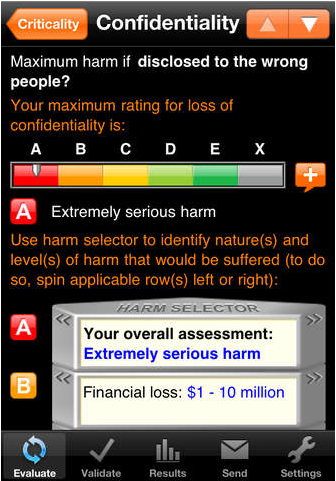
\includegraphics[width=0.4 \textwidth]{./Images/Citicus_MOCA_1.png}
  }
  \caption{Citicus}
  \label{fig:citicus}
\end{figure}

\section{Zusammenfassung}

Im Enterprise Bereich existieren eine Vielzahl an Softwarelösungen fuer Risikomanagement. Die meisten davon sind sehr breit aufgestellt und versuchen möglichst viele Anwendungsfaelle abzudecken. Dadurch sind sie auch eher fuer mittelgrosse bis grosse Firmen geeignet.
Neben diesem Enterprisemarkt gibt es auch einen Markt fuer Teilproblemlösungen. Dafür eignen sich auch durchaus mobile Anwendungen die auf Android oder iOS laufen.


















% --------------------------------------------------------------
\chapter{Risikomanagement im Bereich Service und Data Clouds}
\label{sect:clouds}
\chapter{Risikomanagement im Bereich Service \& Data Clouds}

\section{Einleitung}
Cloud Computing beschreibt das Auslagern von Rechenleistung und Daten in eine externe IT-Infrastruktur, die sogenannte Cloud, welche von einem Provider zur Verfügung gestellt wird. Diese kann entweder zentral oder verteilt auf mehrere Server liegen und bietet dem Benutzer Zugriff auf virtuelle Ressourcen. Für den Benutzer erscheinen Rechenleistung, Datenspeicher, Netzwerkkapazitäten oder gar fertige Softwareprogramme komplett abstrahiert. Die Ressourcen stehen dabei dynamisch zur Verfügung und können je nach momentaner Auslastung angepasst werden. Im Gegensatz zum klassischen "Outsourcing", bei welchem zum Beispiel Rechenleistung eines Dienstleisters exklusiv beansprucht wird, wird die IT-Infrastruktur beim Cloud Computing von mehreren Benutzern gleichzeitig verwendet. Hierbei gibt es allerdings verschiedene sogenannte Deployment Modelle, auf welche später detailliert eingegangen wird. Des Weiteren können auch anhand der Abstraktionsebene verschiedene Service Modelle unterschieden werden. 

\section{IT-Infrastrukturmanagement im Bereich von Service und Data Clouds}
Um besser verstehen zu können, welche Risiken speziell bei Cloud Computing auftreten, wird im Folgenden eine kurze allgemeine Einführung in Cloud Computing und dessen IT-Infrastrukturmanagement gegeben, ehe die einzelnen Risiken aufgeführt und erläutert werden. \cite{koe2013} \cite{haa2013}

\subsection{Charakteristiken des Cloud Computings}
Cloud Computing zeichnet sich durch eine Reihe von Charakteristiken aus, welche vom NIST (National Institute of Standards and Technology) definiert wurden.

\subsubsection{On-demand self-service}
Der Service wird dem Benutzer ohne notwendige Hilfe des Providers zur Verfügung gestellt, so dass dieser jederzeit bei Bedarf auf die benötigten Ressourcen zugreifen kann.

\subsubsection{Broad network access}
Auf die IT-Infrastruktur wird über Netzwerk (Internet) über definierte Schnittstellen zugegriffen werden.

\subsubsection{Resource pooling}
Ressourcen, welche von der Cloud zur Verfügung gestellt werden, können in der Regel von mehreren Benutzern gleichzeitig beansprucht werden. Die einzelnen Komponenten werden so zusammengefasst (gepoolt), dass der Benutzer keinen Einfluss darauf nehmen kann, welche Ressource im zur Verfügung gestellt wird.

\subsubsection{Rapid elasticity}
IT-Komponenten können aufgrund sich schnell ändernder Belastungen sehr flexibel und schnell zusätzlich hinzugefügt oder wieder entzogen werden. Dies garantiert beste Ressourcenauslastung (Effizienz) bei möglichst geringen Überlastungsrisiko.

\subsubsection{Measured service}
Die Nutzung der Cloud Services wird ständig überwacht und gemessen, was sowohl für Provider als auch Nutzer die Benutzung transparent macht.

\subsection{Cloud Computing Service Modelle}
Im Zusammenhang mit Cloud Computing können verschiedene Nutzungsmodelle unterschieden werden. Diese unterscheiden sich vor allem darin, auf welcher Abstraktionsebene die IT-Komponenten der Cloud dem Kunden zur Verfügung gestellt werden. In der Literatur wird meist zwischen drei oder vier unterschieden.

\subsubsection{Infrastructure as a Service - IaaS}
Es werden grundlegende IT-Ressourcen wie Prozessorkapazität, Speicher, Netzwerke usw. zur Nutzung bereit gestellt. Diese Infrastruktur kann vom Kunden genutzt werden um beliebige Betriebssysteme, Software und Netzwerkapplikationen (Host Firewalls) laufen zu lassen. Dieses Service Modell stellt die unterste Abstraktionsebene dar, auf welcher der Kunde am meisten Einfluss auf die dahinter liegende Struktur hat.

\subsubsection{Platform as a Service - Paas}
Dem Benutzer wird eine Plattform zum Entwickeln eigener Software bereit gestellt. Diese Plattform bietet definierte Programmiersprachen, Libraries und Tools um die Softwareentwicklung zu unterstützen.

\subsubsection{Software as a Service - SaaS}
Bei diesem Service Modell kann der Benutzer fertige Software Applikationen nutzen, dabei bleibt die zugrunde liegende Infrastruktur zur Gänze verborgen. Dieses Modell stellt die oberste Abstraktionsebene dar, auf welcher der Kunde lediglich über definierte Schnittstelle die Services von bereits fertig implementierter Software nutzt.

\subsubsection{Business Process as a Service - BPaaS}
Dieses Service Modell wird nicht immer extra angeführt. Es beschreibt im Prinzip die Abbildung eines ganzen Business Prozesses bestehend aus mehreren Komponenten als SaaS.

\subsection{Deployment Modelle}
Ein weiteres wichtiges Unterscheidungsmerkmal verschiedener Cloud Service Provider sind die unterschiedlichen Deployment Modelle. Diese sind vor allem für die spätere Risikoidentifikation interessant, da hier beschrieben wird, wer Zugriff auf die Daten in der Cloud hat. Die beiden wichtigsten Modell sind "Private Cloud" und "Public Cloud" wobei in der Literatur manchmal auch noch "Community Cloud" und "Hybrid Cloud" angeführt werden.

\subsubsection{Private Cloud}
Bei diesem Modell steht die komplette Cloud Infrastruktur einer einzigen Organisation exklusiv zur Verfügung.

\subsubsection{Community Cloud}
Bei der Community Cloud stehen die einzelnen Cloud Komponenten einer definierten Gemeinschaft zur Verfügung, welche gemeinsame Interessen hinsichtlich Sicherheitsanforderungen, Policy usw. verfolgt.

\subsubsection{Public Cloud}
Die Cloud Infrastruktur steht der Öffentlichkeit zur Verfügung und kann von jedem frei benutzt werden.

\subsubsection{Hybrid Cloud}
Dabei handelt es sich um eine Kombination aus zwei oder mehr der oben genannten Modelle.

\section{Typische Risiken bei modernen Service \& Data Clouds}
Im folgenden Abschnitt werden typische Risiken, welche sich aus der speziellen Struktur von Cloud Computing Services ergeben erläutert. Aufgrund der Auslagerung von Rechenkapazitäten oder Datenspeicher entsteht eine gewisse Abhängigkeit vom Cloud Computing Service Provider. Diese Abhängigkeiten können zu verschiedensten Risiken führen. Ein weiterer wichtiger Faktor für die Entstehung von Risiken ist die Undurchsichtigkeit der Datenstruktur einer Cloud Plattform.  

\subsection{Security}
Je nach Deployment Modell wird jegliche Kontrolle über die IT-Infrastruktur an den Provider abgegeben. Beim Software as a Service Modell muss der Benutzer den Sicherheitsrichtlinien des Providers durch alle Ebenen hindurch von Betriebssystem über Netzwerk bis hin zur Software vertrauen. Beim Platform as a Service Modell kann zwar mehr Einfluss auf verwendete Sicherheitsmechanismen genommen werden, allerdings wird auch hier ein Großteil der Kontrolle an den Provider abgegeben. Als zusätzliches Risiko kommt hinzu, dass gerade große Cloud Plattformen ein sehr interessantes Ziel für potentielle Hacker Angriffe sind, da hier meistens sehr große Datenmengen auf einmal gestohlen werden können. Es können zwar bestimmte Vereinbarungen hinsichtlich Security vertraglich geregelt werden, letztendlich ist man aber auf die implementieren Mechanismen des Providers angewiesen und gibt die eigene Kontrollmöglichkeit weitgehend aus der Hand.  \cite{bro2008} 

\subsection{Ausfall}
Durch Nutzung von Cloud Computing entstehen nicht beeinflussbare Risiken bezüglich Ausfall des Cloud Services oder generellere Nicht-Erfüllung der zugesicherten Nutzungsbandbreite und Datenverlust. Es ist daher äußerst wichtig, solche Ausfälle im Vorhinein genauestens vertraglich zu erfassen um im Schadensfall etwaige Ausgleichszahlungen zu erhalten. Dazu muss genau abgeschätzt werden, welches Schadenausmaß ein etwaiger Ausfall annehmen kann und wie wahrscheinlich dieser ist. Der Kunde muss bei der Ausfallswahrscheinlichkeitsminimierung wiederum den Mechanismen des Provider vertrauen ohne darauf signifikant Einfluss nehmen zu können. Dies beinhaltet auch etwaige Recovery Mechanismen.  

\subsection{Supply-Chain Risiken}
Cloud Computing Provider greifen für die Bereitstellung ihrer Services selbst oft auf Drittanbieter zurück, welche wiederum andere Dienstleister einbeziehen. So können komplexe sogenannte "Supply-Chains" entstehen, welche aufgrund der unzähligen einzelnen Sub-Unternehmen ein schwer zu kalkulierendes Risiko darstellen können. Ein Ausfall einer einzelnen Komponente kann unter Umständen die ganze Supply-Chain beeinträchtigen oder sogar zum einem Totalausfall führen.  \cite{haa2013}

\subsection{Veränderungen}
Cloud Computing Plattformen unterliegen wie jede andere Firma im Technologie Bereich ständigen Veränderungen. Diese Veränderungen können sich auf die Services oder deren Preise auswirken. So kann beispielsweise ein neues Business Modell oder neue firmenpolitische Strategien die angebotenen Services einschränken oder sogar teilweise abschaffen. Des Weiteren können sich solche Entscheidungen auch auf die Verfügbarkeit oder Kosten auswirken. Hier ist es wiederum wichtig, den Umfang und eine detaillierte Beschreibung der benötigten Services in Verträgen festzuhalten. \cite{mos2011}


\section{Risiken im Bereich Big Data}
Ein zentrales Thema bezüglich Risikomanagement in Data und Service Cloud Systemen ist der Umgang mit Daten. Die teilweise undurchsichtigen Strukturen von Cloud IT-Infrastrukturen erschweren es den Überblick über Freigabe, Standort und Sicherheit von Daten zu behalten. Diese Tatsache ergibt sich aufgrund der Resource Pooling Charakteristik von Cloud Services. Dieses Konzept hat zur Folge, dass man als Kunde keinen Einfluss darauf hat wo die eigenen Daten gespeichert werden. Diese Undurchsichtigkeit bringt einige Risiken mit sich, welche im Folgenden erläutert werden. 

\subsection{Internal Segmentation}
Cloud Provider, welche nicht Private Cloud als Deployment Modell verwenden bieten ihre Dienste mehreren Organisationen an. Aufgrund der oft undurchsichtigen zugrunde liegenden Datenstruktur besteht das Risiko, das geheime Daten einer Organisation einer anderen fälschlicher Weise zugänglich gemacht werden. Dies kann entweder aufgrund interner Fehler oder aber auch absichtlich durch gezielte Hacker Angriffe geschehen. \cite{mos2011}

\subsection{E-Discovery}
Da die Daten auf dem System des Providers gespeichert werden, begibt man diese in den rechtlichen Geltungsbereich des Providers. Wenn gegen diesen nun aufgrund strafrechtlicher Aktionen Untersuchungen vorgenommen werden, kann es sein, dass nicht nur die Daten des Providers, sondern auch die Daten der Nutzer offen gelegt werden müssen. Dies kann auch dann der Fall sein, wenn der Nutzer nur teilweise oder gar nicht in die Untersuchungen involviert ist. \cite{mos2011}

\subsection{Datenschutz}
Wenn die Daten auf einer undurchsichtigen Cloud Infrastruktur gespeichert werden, welche dem Open Data Prinzip obliegt, so sind diese für jedermann zugänglich. Der Benutzer sollte daher darauf achten, keine kritischen oder personenbezogenen Daten, welche aus datenschutzrechtlichen Gründen nicht öffentlich gemacht werden dürfen, auf so einer Plattform zu speichern. Doch auch im Falle einer Closed Data Struktur besteht aufgrund der vorher genannten Risiken die Gefahr, dass die Daten an die Öffentlichkeit gelangen. Dies kann zum Beispiel auch daran liegen, dass gewisse Big Data Systeme wie zum Beispiel Hadoop nicht von Anfang an darauf ausgelegt wurden, geheime Unternehmensdaten zu speichern. Es ging am Anfang einfach nur darum, enorm große, unstrukturierte Datenmengen verteilt speichern zu können. Diese Design Entscheidungen machen es teilweise schwierig im Nachhinein bestimmte Sicherheitsmechanismen zu implementieren. \cite{haa2013}

\subsection{Verfügbarkeit}
Daten, welche auf einem Cloud Provider gespeichert sind obliegen dessen Verantwortung. Dies kann zu Problemen führen, wenn dieser zum Beispiel von einer anderen Organisation aufgekauft wird oder selber in Konkurs geht. Für diese Fälle muss unbedingt im Vorhinein eine Backup Strategie überlegt werden. Des Weiteren müssen auch Katastrophenfälle und die danach eventuell notwendige Daten Recovery berücksichtigt werden. \cite{mos2011}

\section{Risiken aus Provider-Sicht}
Auch aus der Sicht von Cloud Providern ergeben sich Risiken, welche die spezielle Struktur von solchen Plattformen als Ursache haben.

\subsection{Hacker Attacken}
Wie schon weiter vorher erwähnt sind vor allem Cloud Plattformen ein begehrtes Ziel für Hacker Angriffe. Dies liegt zum einen daran, dass hier sehr viele Daten gespeichert werden. Zum anderen müssen Cloud Service Provider ihre Schnittstellen für das Internet und die breite Öffentlichkeit zugänglich machen, was es potentiellen Hackern erleichtert in das System einzudringen. \cite{mos2011}

\subsection{Unbemerkter Datenverlust}
Allzu oft kommt es vor, dass Daten gestohlen werden, ohne dass die betroffene Organisation das merkt und den Cloud Provider davon informieren kann. Dieser kann daher erst sehr verspätet darauf reagieren und ein Durchdringen der Attacke an die Öffentlichkeit, was mit einem erheblichen Image Schaden verbunden ist, nicht mehr verhindern.\cite{mos2011}

\subsection{Verteilte Datenspeicher}
Ein Cloud System verteilt die Daten auf mehrere Server. Dabei muss immer darauf geachtet werden, welche Daten in welche Region oder in welches Land gespeichert werden, da es in diesem Bereich oftmals rechtliche Vorgaben seitens des Gesetzes oder auch Vorgaben der Organisation geben kann. \cite{mos2011}





% --------------------------------------------------------------
\chapter{Risikomanagnement im Kontext von Smart Technologien}
\label{sect:relevance}

\section{Neue IT-Risiken durch Smart Technologies (Internet of Things)}



Es ist nur mehr eine Frage der Zeit, bis alle „Dinge“ mit dem World Wide Web kommunizieren und Daten austauschen. Wie schön dies auch klingt und unser Leben dadurch auch in gewisser Weise erleichtert wird, verbergen sich hinter diesen Maßnahmen auch Risiken, die zum Teil auch neu sind. Diese Risiken bestehen sowohl für Unternehmen als auch für Verbraucher. Jedes Gerät, dass eine Internetverbindung hat, ist zugleich eine offene Tür für Angreifer. Einige dieser Geräte haben Betriebssysteme wie Linux oder Android installiert und bringen auch dieselben Stärken und Lücken mit.
Überwachung spielt hier eine sehr wichtige Rolle. Wenn zu bestimmten Zeitpunkten auffällige Geschehnisse auftreten, könnte dies ein Indiz dafür sein, dass etwas nicht stimmt. Mit einer Überwachungssoftware würde dieser Prozess einfach gestoppt werden. 
\\
\\
Durch die gute Vernetzung der intelligenten Technologien, kann sobald sich ein Virus in ein Gerät eingenistet hat, sich ganz einfach auf andere Geräte verbreiten. Im Falle der Datenspionage kann die Privatsphäre noch stärker verletzt werden. Da die Geräte vernetzt sind und jedes davon verschiedene User Informationen enthalten, ist es für den Angreifer noch leichter alle Daten auf einen Schlag zu bekommen.
\\
\\
Wenn wir die Gruppe Wearables betrachten gibt es Geräte die wichtige Funktionen Im menschlichen Körper steuern und dadurch unterstützen. Dies bringt ein Lebensgefährliches Risiko mit. Sei es ferngesteuerte Insulinpumpen oder Geräte für die Stimulation des Herzens. Hier dürfen keine Sicherheitslücken existieren, da ansonsten die Personen die diese Wearables tragen und benützen, in Lebensgefahr gebracht werden.
\\
\\
Unternehmen, die den Smart Technology Trend mit dem sogenannten „Bring your own Device“ – Betriebsvereinbarungen verfolgen, gehen ebenfalls ein hohes Sicherheitsrisiko ein. Private Geräte können nur teilweise überwacht und kontrolliert werden, wodurch sensible Unternehmensdaten in falsche Hände geraten können. Um einen sinnvollen Einsatz der Smart Technologies im Unternehmen zu gewährleisten, müssen diese auch immer online sein, da ansonsten mit Ausfällen ein Schaden angerichtet werden könnte.
\\
\\
\begin{figure}[hbtp]
\centering
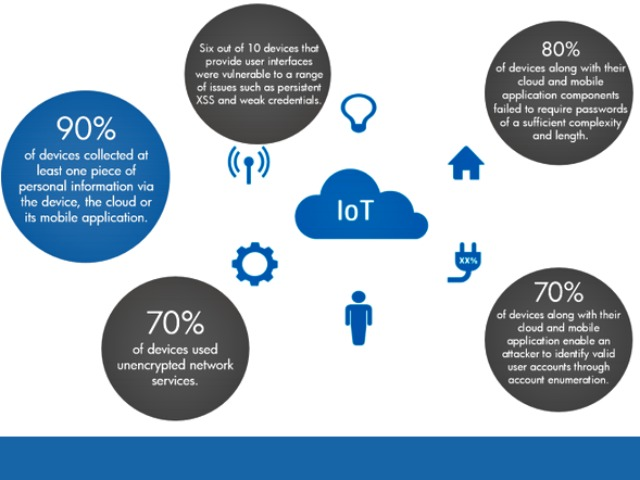
\includegraphics[scale=0.5]{hp-iot-security.jpg}
\caption{HP Studie Internet of Things (http://www8.hp.com/h20195/V2/GetPDF.aspx/4AA5-4759ENW.pdf)}
\end{figure}

\section{Spezifische Bereichsrisiken}

\subsection{Smart Home}

\textbf{Elektronik:} Intelligente Haushaltsgeräte sowie Beleuchtungen und Fenster schaffen zusätzliche Belastung in der Hauselektronik. Smarte Technologien die über Web-basierende Apps angesteuert werden, sind anfällig für Überspannungen und Blitzschlag. Diese haben konsequenterweise Einfluss auf das gesamte elektrische System im Haus. Das Motherboard des Steuergerätes der Smart Home Technologie könnte dadurch auch einen Schaden bekommen. Hohe Reparaturkosten wären dann die Folgen.
\\
\\
\textbf{Web Sicherheit:} Die Verwendung moderner und innovativer Technologie Zuhause, erleichtert uns das Leben und kann auch viel Geld einsparen. Eine Waschmaschine die mit dem WLAN verbunden ist und den Waschgang erst dann startet wenn der Strompreis am günstigsten ist, würde im Haushalt einiges an Geld einsparen. Jedoch jedes Gerät, das mit dem Internet verbunden wird, wird Möglicherweise auch zugänglich für andere. 
Da diese Systeme zurzeit von kleineren Unternehmen entwickelt werden, kann die Sicherheit schwach ausfallen.
\\
\\
\textbf{Privatsphäre:} Nachdem ein Smart Home System gehackt wurde, besteht natürlich auch das Risiko, dass die Privatsphäre verletzt werden kann. Es kann Zugang zu den Kameras, zum Smart TV oder Babyfon verschafft werden. In den USA gab es einen Vorfall, wo ein Hacker das Kind durch das Babyfon beschimpft hat.\footnote{http://www.n24.de/n24/Wissen/Technik/d/3379940/-wach-auf--du-kleine-schlampe-.html}
Gewohnheiten sowie Urlaubsaufenthalte können ausgeforscht werden, was dazu führt, dass Kriminelle auch physischen Schaden anrichten können.
\\
\\
\textbf{Versicherungsdeckung:} Wenn Smart Home Technologies verwendet werden, muss auch über eine Fern Überwachung gedacht werden. Dies dient nicht nur zur persönlichen Sicherheit sondern auch für die Versicherungsdeckung. Es müssen über Firewalls und Passwortschutz nachgedacht werden.

\subsection{Smart Factory (Industrie 4.0)}

So groß die Risiken sind so groß sind auch die Vorteile. Maschinen und Bauteile können sich verständigen, dadurch kann extrem genau in der Produktion kalkuliert werden. Das bringt Ressourceneffizienz weniger Materialeinsatz und eine bessere Ökobilanz. 
Durch die Vernetzung der Einheiten in der Produktion, sind kleinere Subsysteme immer enger gekoppelt und voneinander Abhängig. Dadurch steigt die Komplexität und parallel auch das Risiko.
\\
\\
Während der Einsatz von intelligenter Industrie den menschlichen Fehler als Risikofaktor senkt, könnten bei Problemen mit den Maschinen menschlicher Einsatz benötigt werden. Diese Personen müssen bestimmte Qualifikationen und Fertigkeiten besitzen um derartige Probleme lösen zu können. In so einem Fall kann möglicherweise die ganze Produktionskette lahmgelegt werden. Der "menschliche Faktor" geht sozusagen verloren. Zum Beispiel: Was passiert wenn eine Gasleitung undicht wird und es ist keiner da der es bemerkt. Solche Risiken müssen aufgespürt werden und in den Designprozess mit einfließen.
\\
\\
Das finanzielle Risiko spielt demnach auch eine wesentliche Rolle. Wenn neue intelligente Technologien in der Industrie eingesetzt werden, stellt sich die Frage ob es die Mitarbeiter dazu gibt, die diese Geräte zu bedienen wissen. Es werden eventuell neue Leute mit neuen Fertigkeiten benötigt die mehr Kosten. Was passiert wenn die Integration der intelligenten Maschinen in den Arbeitsablauf fehlschlägt. Das Unternehmen könnte die geforderte Produktionsmenge nicht mehr einhalten. Dies könnte im weiteren zu einer Rufschädigung führen, was für ein Unternehmen das schlimmste wäre.
\\
\\
Die bisher besprochenen Fälle können bei gut durchdachtem Risikomanagement kalkuliert und bewältigt werden. Was ist jedoch wenn ein Hacker oder ein Mitarbeiter die intelligenten Maschinen mit einem Virus infiziert. Dies würde alle schlimmen Szenarien ermöglichen. Herunterfahren von Maschinen, Produktionsdefekte, Umweltschäden bis hin zur Wirtschaftsspionage wichtiger Prozesse und Daten. Der Erholungsprozess eines Unternehmens von solch einer Attacke könnte über Jahre hinweg andauern.

Versicherbarkeit?
Hohe Wartungskosten

\subsection{Smart Car}

Autos werden immer intelligenter. Selbstparksysteme und Abstandsregeltempomaten sind bereits auf dem Markt. Autos kommunizieren mit anderen Autos und kontrollieren das Fahrzeug für mehr Sicherheit und Bequemlichkeit. Diese neuen intelligenten Technologien kommen bald in die Massenproduktion und werden unvermeidlich. Wie auch in den anderen Bereichen, bietet diese Innovation reichlich Platz an Risiken.
Im Jänner 2015 wurde im System „ConnectedDrive“ von BMW eine Sicherheitslücke entdeckt. Diese Lücke erlaubte die Autos mit dem Mobiltelefon per GSM-Funk zu öffnen. Der Grund dafür war die unverschlüsselte Kommunikation, welche BMW aber abstreitet. Es waren 2,2 Millionen Autos davon betroffen und der Fehler existierte über Jahre inweg. inweg\footnote{http://www.spiegel.de/auto/aktuell/adac-entdeckt-it-sicherheitsluecke-bei-bmw-connected-drive-a-1015819.html}
\\
\\
Assistenzsysteme, die für Bremsen und halten der Spur zuständig sind, können von außen manipuliert werden. Diese Manipulation hat zur Folge, dass falsche Signale simuliert werden und so die Kontrolle des Autos in andere Hände übergehen kann. Je stärker die Kopplung der Systeme zueinander steht, desto leichter ist es für Eindringlinge das System zu überlisten.
\\
\\
Mit der Einführung des Smart Cars muss die Gesellschaft auch lernen umzudenken. Die Sicherheit, Unfälle durch menschlichen Fehler zu vermeiden steigt enorm, jedoch müssen Fahrzeuge nun vor Hackangriffen geschützt werden. Im Falle eines Unfalles, der durch einen Hackangriff verursacht wurde, stellt sich die Frage, wer die Schuld trägt? Diese und weitere Fragen müssen sorgfältig behandelt und geklärt werden.
\\
\\
Der Umgang mit persönlichen Daten spielt auch eine sehr wichtige Rolle. Autos speichern und übertragen viele persönliche Daten wie Bewegungsprofile, Fahrweise, Verbrauch, Telefonbücher und sogar Kreditkartendaten bei automatisierter Bezahlung von Parkgebühren. Diese Daten sind für Cyberkriminelle von hohem Wert.
\\
\\
Da bei Smart Cars zwei unterschiedliche Branchen aufeinandertreffen, bringt dies auch ein gewisses Risiko mit.  Während in der IT monatliche Zyklen Standard sind, ist man in der Autoindustrie eher den Jahreszyklus gewöhnt. 

\section{Best Practices beim Management von Smart-Technology-Risiken}

Eine routinierte Sicherheitsüberprüfung auf den Geräten und den verbundenen Komponenten ist das A und O. Aufgrund der Menge der Geräte muss diese automatisiert erfolgen. Die zu überprüfenden Komponenten sind:

\begin{itemize}
\item Web-Schnittstelle
\item Netzwerkübertragung
\item Ports
\item Authentifizierung / Autorisierung
\item Cloud communication
\end{itemize}
Es müssen Securiy-Policies entwickelt werden die jedes einzelne Gerät erfüllen muss. Wenn diese Standards einmal aufgesetzt und danach aktuell gehalten werden, ist das eine hohe Risikominimierung.
\\
\\
Damit die Sicherheit auch Gewährleistet ist, muss dieser Aspekt im ganzen Product-Lifecycle angewandt werden. Die frühe Begutachtung von Prozessergebnissen hält das Risiko gering. Softwareupdates sind somit bei Auftreten von Fehlern sehr wichtig. Wenn diese Updates schnell und routiniert eingespielt werden, bleibt das System bzw. die Geräte immer auf dem neuesten Sicherheitsstand.


\bibliographystyle{acm}
\bibliography{risk2015}

\end{document}
